\newcommand*{\DatabaseOverviewPath}{04-framework/02-implementation/01-database}

% --- SUBSECTION DATABASE ---
\subsection{Database overview\label{sec:database-overview}}
All the data acquired or generated is stored in a single relational database called \inlinecode{sentiment\_db}. 
The logical view of the database is shown in Figure \ref{fig:db-schema}. 
In favor of clarity parts considered inconsequential to sentiment analysis processes are not disclosed. 
Those include, but are not limited to: django sessions, brands etc.
\usetikzlibrary{positioning,shapes,arrows}

\tikzstyle{table}=[rectangle, rectangle split, rectangle split parts=2, rounded corners=2pt, draw=black,fill=white, inner sep=0.2cm, font=\scriptsize\mdseries]
\tikzstyle{line}=[>-, thick, dashed]
        
\begin{figure}[H]
\centering  
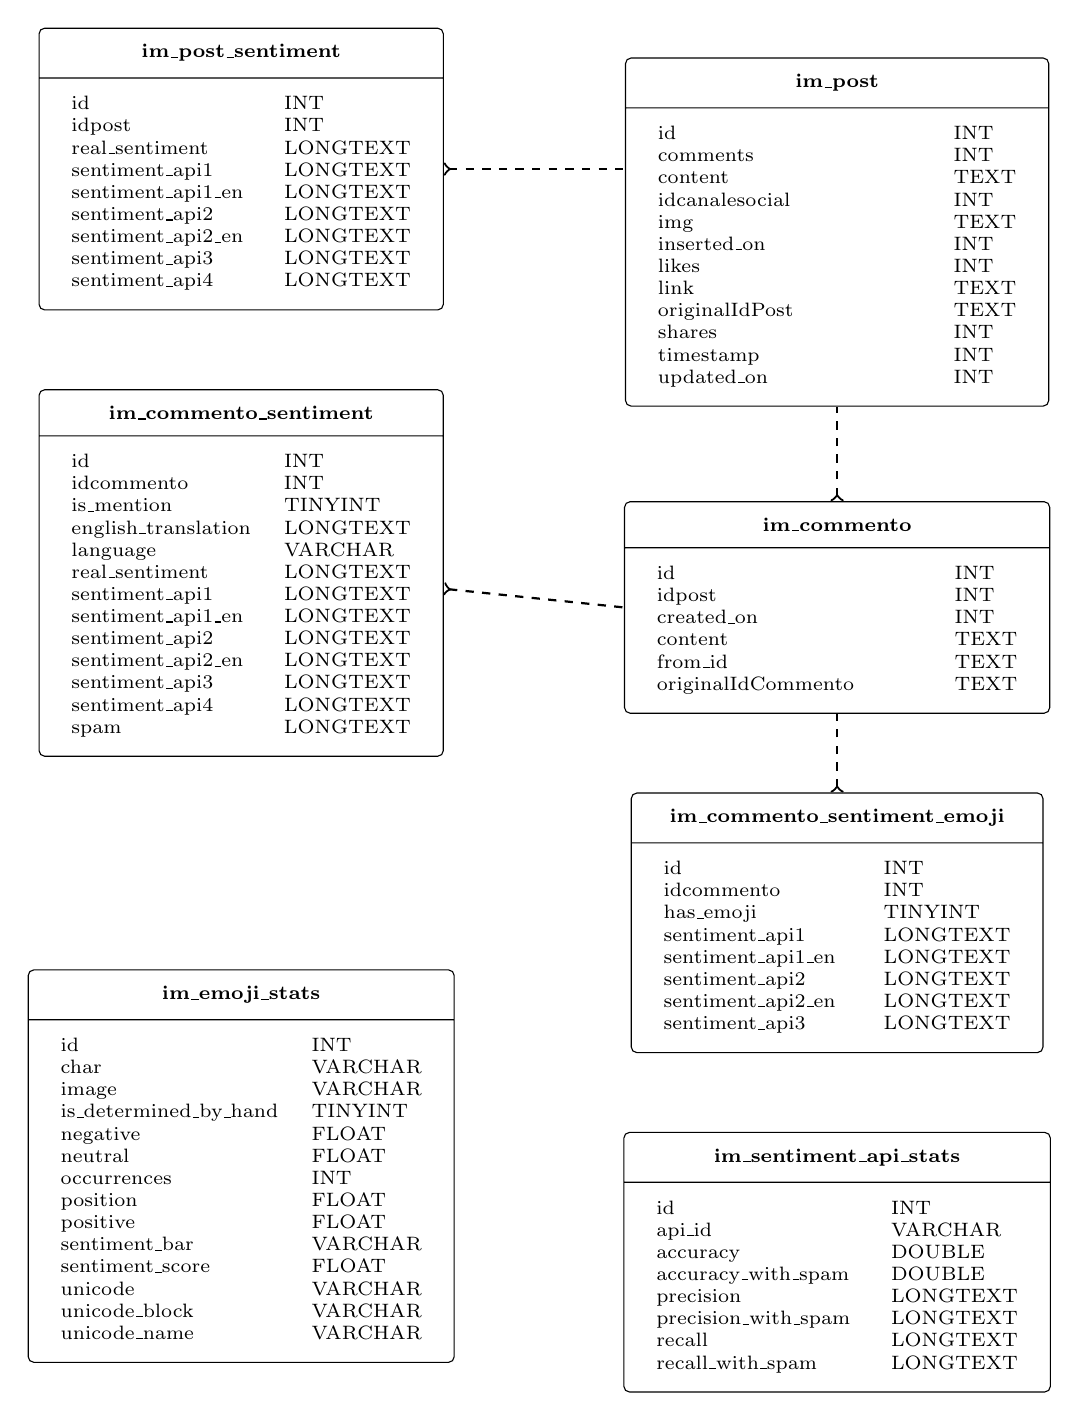
\begin{tikzpicture}[node distance=1cm]
\onehalfspacing

    \node (im-post) [table]{
        \textbf{im\_post}
        \nodepart{second}
            \tabular{ll} 
            id & INT \\ 
            comments & INT \\ 
            content & TEXT \\ 
            idcanalesocial & INT \\ 
            img & TEXT \\ 
            inserted\_on & INT \\ 
            likes & INT \\ 
            link & TEXT \\ 
            originalIdPost \ \ \ \ \ \ \ \ \ \ \ \ \ \ \ \ \ & TEXT \\
            shares & INT \\
            timestamp & INT \\
            updated\_on & INT \\                        
            \endtabular
    };

    \node (im-post-sentiment) [table, left=of im-post, yshift=0.8cm, xshift=-1.3cm]{
        \textbf{im\_post\_sentiment}
        \nodepart{second}
            \tabular{ll}                    
            id & INT \\
            idpost & INT \\
            real\_sentiment & LONGTEXT \\
            sentiment\_api1 & LONGTEXT \\
            sentiment\_api1\_en \ & LONGTEXT \\
            sentiment\_api2 & LONGTEXT \\
            sentiment\_api2\_en & LONGTEXT \\
            sentiment\_api3 & LONGTEXT \\
            sentiment\_api4 & LONGTEXT \\
            \endtabular
    };

    \node (im-commento) [table, below=of im-post,yshift=-0.2cm ]{
        \textbf{im\_commento}
        \nodepart{second}
            \tabular{ll}                    
            id & INT \\
            idpost & INT \\
            created\_on & INT \\
            content & TEXT \\
            from\_id & TEXT \\
            originalIdCommento \ \ \ \ \ \ \ \ \ & TEXT \\
            \endtabular
    };

    \node (im-commento-sentiment) [table, below=of im-post-sentiment]{
        \textbf{im\_commento\_sentiment}
        \nodepart{second}
            \tabular{ll}                    
            id & INT \\
            idcommento & INT \\
            is\_mention & TINYINT \\
            english\_translation & LONGTEXT \\
            language & VARCHAR \\
            real\_sentiment & LONGTEXT \\
            sentiment\_api1 & LONGTEXT \\
            sentiment\_api1\_en & LONGTEXT \\
            sentiment\_api2 & LONGTEXT \\
            sentiment\_api2\_en & LONGTEXT \\
            sentiment\_api3 & LONGTEXT \\
            sentiment\_api4 & LONGTEXT \\
            spam & LONGTEXT \\
            \endtabular
    };

    \node (im-commento-sentiment-emoji) [table, below=of im-commento]{
        \textbf{im\_commento\_sentiment\_emoji}
        \nodepart{second}
            \tabular{ll}                    
            id & INT \\
            idcommento & INT \\
            has\_emoji & TINYINT \\
            sentiment\_api1 & LONGTEXT \\
            sentiment\_api1\_en & LONGTEXT \\
            sentiment\_api2 & LONGTEXT \\
            sentiment\_api2\_en  \ \ & LONGTEXT \\
            sentiment\_api3 & LONGTEXT \\
            \endtabular
    };

    \node (im-sentiment-api-stats) [table, below=of im-commento-sentiment-emoji]{
        \textbf{im\_sentiment\_api\_stats}
        \nodepart{second}
            \tabular{ll}                    
            id & INT \\
            api\_id & VARCHAR \\
            accuracy & DOUBLE \\
            accuracy\_with\_spam & DOUBLE \\
            precision & LONGTEXT \\
            precision\_with\_spam \ & LONGTEXT \\
            recall & LONGTEXT \\
            recall\_with\_spam & LONGTEXT \\
            \endtabular
    };

    \node (im-emoji-stats) [table, below=of im-commento-sentiment, yshift=-1.7cm]{
        \textbf{im\_emoji\_stats}
        \nodepart{second}
            \tabular{ll}                    
            id & INT \\
            char & VARCHAR \\
            image & VARCHAR \\
            is\_determined\_by\_hand & TINYINT \\
            negative & FLOAT \\
            neutral & FLOAT \\
            occurrences & INT \\
            position & FLOAT \\
            positive & FLOAT \\
            sentiment\_bar & VARCHAR \\
            sentiment\_score & FLOAT \\
            unicode & VARCHAR \\
            unicode\_block & VARCHAR \\
            unicode\_name & VARCHAR \\
            \endtabular
    };

    \draw[line] (im-post-sentiment.east) -- ([yshift=0.8cm] im-post.west);
    \draw[line] (im-commento.north) -- (im-post.south);
    \draw[line] ([yshift=-0.2cm] im-commento-sentiment.east) -- (im-commento.west);
    \draw[line] ( im-commento-sentiment-emoji.north) |- (im-commento.south);
   
\end{tikzpicture}
  \caption{Database schema}
  \label{fig:db-schema}
\end{figure}

As previously stated, we have extended and built our framework on top of a preexisting relational MySQL database schema which came with a set of specifications which were adopted and applied to \inlinecode{sentiment\_db}.
Using a version of MySQL greater or equal to 5.5.3 was a hard constraint because in that release MySQL introduced support for \inlinecode{uft8mb4} encoding.  
As opposed to \inlinecode{uft8}'s three bytes per character maximum, 
\inlinecode{uft8mb4} uses a maximum of four bytes per character making it fully compatible with \inlinecode{uft8} and, most importantly, able to correctly encode and store emojis.
It is worth mentioning that only two data tables that were a part of the original database were used and those are \inlinecode{im\_commento} and \inlinecode{im\_post}.

For the sake of completeness, following tables contain details and field descriptions of used data tables. 

\begin{table}[H]
\centering
\onehalfspacing

\begin{tabularx}{0.95\textwidth}{ l || c | X }
	\hline
	\multicolumn{3}{l}{ \textbf{im\_post} } \\
	\hline

 	\textbf{id} & INT & PRIMARY KEY \\  
	comments & INT & number of comments the post has \\  
	content & TEXT & post's content \\  
	idcanalesocial & INT & FORGEIN KEY to im\_canalesocial: \newline field links to the post's social media account \\  
	img & TEXT & url to post's accompanying photo \\  
	inserted\_on & INT & timestamp when the record was inserted \\  
	likes & INT & number of likes the post has \\  
	link & TEXT & url to the post on a social media site \\  
	originalIdPost \ \  & TEXT & identifier used on its social media site \\ 
	shares & INT & number of shares the post has \\ 
	timestamp & INT & timestamp when the post was created \\ 
	updated\_on & INT & timestamp when the record was updated \\ 
  
	\hline
\end{tabularx}
\caption{Overview of \inlinecode{im\_post} database table}
\label{tab:im-post}

\end{table}
\begin{table}[H]
\centering
\onehalfspacing

\begin{tabularx}{0.95\textwidth}{ l || c | X }
	\hline
	\multicolumn{3}{l}{ \textbf{im\_commento} } \\
	\hline

 	\textbf{id} & INT & PRIMARY KEY \\  
	idpost & INT & FORGEIN KEY to im\_post: \newline field links to the comment's post \\  
	created\_on & INT & timestamp when the comment was created \\
	content & TEXT & comment's content \\
	from\_id & TEXT & commentator's id \\
	originalIdCommento & TEXT & identifier used on its social media site \\
 
	\hline
\end{tabularx}

\caption{Overview of \inlinecode{im\_commento} database table}
\label{tab:im-commento}

\end{table}
\newpage

As mentioned, emojis play a big role in determining sentiment of a comment. 
Since none of the APIs took them into account, we used sentiment scores from \emph{Emoji Sentiment Ranking}\footnote{http://kt.ijs.si/data/Emoji\_sentiment\_ranking} published as a part of a sentiment analysis study\cite{Kralj2015emojis},  and imported them into the database table \inlinecode{im\_emoji\_stats} whose details are shown in Table \ref{tab:im-emoji-stats}.  
However, not all emojis or emoticons that occurred in our data set were included in the study (e.g. 📘 🍾 🙂 🙄 🕶 :) :D ).
Which means they had to be manually inserted in the db. 
Their sentiment scores were determined by finding a similarly defined emoji and making the assumption that they had the same, or at least similar, sentiment. 
%All emojis that were inserted by hand are marked by a true value in  \inlinecode{is\_determined\_by\_hand} column.
For example, green book's (📗) sentiment score was used in place for the missing blue book emoji (📘). 
An example of missing inserted emojis and their similar counterparts can be found in Table \ref{tab:inserted-emoticons}
\begin{table}[H]
\centering
\onehalfspacing

\begin{tabularx}{0.95\textwidth}{ c | c | c | X }
	\hline
	\textbf{Inserted icon} & \textbf{Similar icon} & \textbf{Sentiment score} & \textbf{Unicode name} \\  
 	\hline
	📘        & 📗 & 0.491 & Blue book \\
	🙂        &  ☺ & 0.72 & Slightly smiling face \\
	🕶        & 😎 & 0.491 & Dark sunglasses \\
	:-) :) =) &  ☺ & 0.657 & Smiley face \\
	:*        & 😘 & 0.71 & Kiss face \\
\textless3    & ❤  &  0.657 & Heart  \\
	\hline
\end{tabularx}

\caption{Example of inserted emojis into \inlinecode{im\_emoji\_stats} database table}
\label{tab:inserted-emoticons}

\end{table}
\begin{table}[H]
\centering
\onehalfspacing

\begin{tabularx}{0.95\textwidth}{ l || c | X }
	\hline
	\multicolumn{3}{l}{ \textbf{im\_emoji\_stats} } \\
	\hline
 	\textbf{id} & INT & PRIMARY KEY \\  
	char & VARCHAR &  emoji  characers \\ 
	is\_determined\_by\_hand & TINYINT & boolean variable that denotes if emoji or emoticons were added by hand or used stats from the study \emph{Emoji Sentiment Ranking} \\ 
	negative & FLOAT &  how negative is the emoji $\in [0,1]$ \\ 
	neutral & FLOAT &  how neutral is the emoji $\in [0,1]$ \\ 
	occurrences & INT & number of occurrences of the emoji in all comments in our dataset \\ 
	positive & FLOAT & how positive is the emoji $\in [0,1]$ \\ 
	sentiment\_score & FLOAT & overall sentiment score $\in [-1,1]$ \\ 
	unicode & VARCHAR & unicode codepoint of the emoji \\ 
	unicode\_block & VARCHAR & general category an emoji falls into \\ 
	unicode\_name & VARCHAR & descriptive name of the emoji \\ 
	\hline
\end{tabularx}

\caption{Overview of \inlinecode{im\_emoji\_stats} database table}
\label{tab:im-emoji-stats}

\end{table}

Tables \ref{tab:im-commento-sentiment}, \ref{tab:im-post-sentiment}, \ref{tab:im-commento-sentiment} and \ref{tab:im-sentiment-api-stats}  

Why json when it violated the 1NN rule? already in mysql, will eventually support json, and easily movable to nosql db, or even elastic search. 

Out of the table columns listed above, the following are in json format but stored as lontext:



\newsavebox\sentimentexample
\newsavebox\spamexample

\begin{lrbox}{\sentimentexample}
\begin{lstlisting}[
style=json,
label={lst:default-sentiment-json-table}]
{
  "sentiment_label": "",
  "sentiment_stats": {
      "positive": 0,
      "negative": 0
      "neutral" : 0
  }
}
\end{lstlisting}
\end{lrbox}

\begin{lrbox}{\spamexample}
\begin{lstlisting}[
style=json,
label={lst:default-spam-json}]
{
  "type": "", 
  "is_spam": false
}
\end{lstlisting}
\end{lrbox}

\begin{table}[H]
\centering
\onehalfspacing

\begin{tabularx}{0.95\textwidth}{ m{35mm} || c | X }
	\hline
	\multicolumn{3}{l}{ \textbf{im\_commento\_sentiment / im\_commento\_sentiment\_emoji} } \\ \hline
	\hline
	\textbf{id} & INT & PRIMARY KEY \\ \hline  
    idcommento & INT & FORGEIN KEY to im\_comment: \newline the field points to comment's id \\ \hline  
    is\_mention & TINYINT & boolean variable that denotes if there was a mention of a user in the comment (e.q @Anna) \\ \hline  
    english\_translation & LONGTEXT & Google Translate API's English translation of the content \\ \hline
    language & VARCHAR & Google Translate API's prediction of content's  original language \\ \hline
	real\_sentiment & LONGTEXT & manually determined sentiment\\ \hline
	sentiment\_api1,
	sentiment\_api1\_en, 
	sentiment\_api2, 
	sentiment\_api2\_en,
	sentiment\_api3, 
	sentiment\_api4 & LONGTEXT & 
	\begin{tabular}[t]{ m{60mm}}
		API's sentiment prediction of content in original (English) language. 
		All \inlinecode{sentiment\_api} columns default to:\newline
		\usebox\sentimentexample  
  	\end{tabular}\\ \hline
	spam & LONGTEXT & manually determined whether or not the content is spam\newline defaults to:\newline
\usebox\spamexample  \\ \hline

\end{tabularx}
\caption{Overview of \inlinecode{im\_commento\_sentiment} and \newline \inlinecode{im\_commento\_sentiment\_emoji} database table}
\label{tab:im-commento-sentiment}

\end{table}
\newsavebox\postsentimentexample

\begin{lrbox}{\postsentimentexample}
\begin{lstlisting}[
style=json,
label={lst:default-post-sentiment-json}]
{
  "sentiment_stats": {
    "positive": 9, 
    "negative": 2,
    "neutral": 38, 
    "total": 49
  }, 
  "sentiment_label": "neutral"
  "total_comments": 49,
}
\end{lstlisting}
\end{lrbox}


\begin{table}[H]
\centering
\onehalfspacing

\begin{tabularx}{0.95\textwidth}{ m{35mm} || c | X }
	\hline
	\multicolumn{3}{l}{ \textbf{im\_post\_sentiment} } \\ \hline
	\hline
	\textbf{id} & INT & PRIMARY KEY \\ \hline  
    idpost & INT & FORGEIN KEY to im\_post: \newline the field points to post's id \\ \hline  
    real\_sentiment & LONGTEXT & aggregation over post's comments of: real sentiment data \\ \hline 
	sentiment\_api1,
	sentiment\_api1\_en, 
	sentiment\_api2, 
	sentiment\_api2\_en,
	sentiment\_api3, 
	sentiment\_api4 & LONGTEXT & 
	\begin{tabular}[t]{ m{60mm}}
		aggregation over post's comments of:
		API's sentiment predictions in original (English) language.
		All \inlinecode{sentiment\_api} columns default to:\newline
		\usebox\postsentimentexample 
  	\end{tabular}\\ \hline


\end{tabularx}
\caption{Overview of \inlinecode{im\_post\_sentiment} database table}
\label{tab:im-post-sentiment}

\end{table}
\newsavebox\sentimentstatsexample
\newsavebox\apiid

\begin{lrbox}{\apiid}
\begin{lstlisting}[
style=json,
label={lst:api-id-json}]
 sentiment_api1, 
 sentiment_api1_en, 
 sentiment_api1_emoji,
 sentiment_api1_en_emoji,
 sentiment_api2 ...
\end{lstlisting}
\end{lrbox}


\begin{lrbox}{\sentimentstatsexample}
\begin{lstlisting}[
style=json,
label={lst:sentiment-api-stats-json}]
{
  "positive": 0.5965, 
  "negative": 0.3946,
  "neutral":  0.4578 
}
\end{lstlisting}
\end{lrbox}


\begin{table}[H]
\centering
\onehalfspacing

\begin{tabularx}{0.95\textwidth}{ l || c | X }
	\hline
	\multicolumn{3}{l}{ \textbf{im\_sentiment\_api\_stats} } \\ \hline
	\hline

	\textbf{id} & INT & PRIMARY KEY \\ \hline 
	api\_id & VARCHAR & String identifying API and comment content version used. For example: \newline \usebox\apiid
	 \\ \hline  
    accuracy & DOUBLE & Accuracy of the API excluding comments marked as spam \\ \hline  
    accuracy\_with\_spam & DOUBLE & Accuracy of the API including comments marked as spam \\ \hline 
    
    precision & LONGTEXT & Precision per sentiment label of the API excluding comments marked as spam \\ \hline 
	precision\_with\_spam & LONGTEXT & Precision per sentiment label of the API including comments marked as spam \\ \hline

	recall & LONGTEXT & Recall per sentiment label of the API excluding comments marked as spam \\ \hline 
	recall\_with\_spam & LONGTEXT & Recall per sentiment label of the API including comments marked as spam \newline
	Example of recall and precision column values:\newline
	\usebox\sentimentstatsexample  \\ \hline

\end{tabularx}
\caption{Overview of \inlinecode{im\_sentiment\_api\_stats} database table}
\label{tab:im-sentiment-api-stats}

\end{table}